
\documentclass{beamer}

\mode<presentation> {

% The Beamer class comes with a number of default slide themes
% which change the colors and layouts of slides. Below this is a list
% of all the themes, uncomment each in turn to see what they look like.

%\usetheme{default}
%\usetheme{AnnArbor}
%\usetheme{Antibes}
%\usetheme{Bergen}
%\usetheme{Berkeley}
%\usetheme{Berlin}
%\usetheme{Boadilla}
%\usetheme{CambridgeUS}
%\usetheme{Copenhagen}
%\usetheme{Darmstadt}
%\usetheme{Dresden}
%\usetheme{Frankfurt}
%\usetheme{Goettingen}
%\usetheme{Hannover}
%\usetheme{Ilmenau}
%\usetheme{JuanLesPins}
%\usetheme{Luebeck}
\usetheme{Madrid}
%\usetheme{Malmoe}
%\usetheme{Marburg}
%\usetheme{Montpellier}
%\usetheme{PaloAlto}
%\usetheme{Pittsburgh}
%\usetheme{Rochester}
%\usetheme{Singapore}
%\usetheme{Szeged}
%\usetheme{Warsaw}

% As well as themes, the Beamer class has a number of color themes
% for any slide theme. Uncomment each of these in turn to see how it
% changes the colors of your current slide theme.

%\usecolortheme{albatross}
%\usecolortheme{beaver}
%\usecolortheme{beetle}
%\usecolortheme{crane}
%\usecolortheme{dolphin}
%\usecolortheme{dove}
%\usecolortheme{fly}
%\usecolortheme{lily}
%\usecolortheme{orchid}
%\usecolortheme{rose}
%\usecolortheme{seagull}
%\usecolortheme{seahorse}
%\usecolortheme{whale}
%\usecolortheme{wolverine}

%\setbeamertemplate{footline} % To remove the footer line in all slides uncomment this line
%\setbeamertemplate{footline}[page number] % To replace the footer line in all slides with a simple slide count uncomment this line

%\setbeamertemplate{navigation symbols}{} % To remove the navigation symbols from the bottom of all slides uncomment this line
}

\usepackage[utf8]{inputenc}
\usepackage{graphicx} % Allows including images
\usepackage{booktabs} % Allows the use of \toprule, \midrule and \bottomrule in tables
\usepackage{mathtools}
\usepackage{listings}
\usepackage{color}

\definecolor{codegreen}{rgb}{0,0.6,0}
\definecolor{codegray}{rgb}{0.5,0.5,0.5}
\definecolor{codepurple}{rgb}{0.58,0,0.82}
\definecolor{backcolour}{rgb}{0.95,0.95,0.92}

\lstdefinestyle{mystyle}{
    backgroundcolor=\color{backcolour},   
    commentstyle=\color{codegreen},
    keywordstyle=\color{magenta},
    numberstyle=\tiny\color{codegray},
    stringstyle=\color{codepurple},
    basicstyle=\footnotesize,
    breakatwhitespace=false,         
    breaklines=true,                 
    captionpos=b,                    
    keepspaces=true,                 
    numbers=left,                    
    numbersep=5pt,                  
    showspaces=false,                
    showstringspaces=false,
    showtabs=false,                  
    tabsize=2
}
\lstset{style=mystyle}

\inputencoding{utf8}

%----------------------------------------------------------------------------------------
%	TITLE PAGE
%----------------------------------------------------------------------------------------

\title[Turning Bands]{The Turning Bands Method} % The short title appears at the bottom of every slide, the full title is only on the title page

\author{Péricles Lopes Machado} % Your name
\institute[UFRGS] % Your institution as it will appear on the bottom of every slide, may be shorthand to save space
{
Universidade Federal do Rio Grande do Sul \\ % Your institution for the title page
\medskip
\textit{eu@gogo40.com} % Your email address
}

\date{\today} % Date, can be changed to a custom date

\begin{document}

\begin{frame}
\titlepage % Print the title page as the first slide
\end{frame}

\begin{frame}
\frametitle{Overview} % Table of contents slide, comment this block out to remove it
\tableofcontents % Throughout your presentation, if you choose to use \section{} and \subsection{} commands, these will automatically be printed on this slide as an overview of your presentation
\end{frame}

%----------------------------------------------------------------------------------------
%	PRESENTATION SLIDES
%----------------------------------------------------------------------------------------


%%%%%%%%%%%%%%%%%%%%%%%%%%%%%%%%%%%%%%%%%%%%%%%%%%%%%%%%%%%%%%%%%%%%%%%%%%%%%%%%%%%%%%%%%%%%%%%%%%%%%%%%%%%%%%%%
\section{What is turning bands?} % Sections can be created in order to organize your presentation into discrete blocks, all sections and subsections are automatically printed in the table of contents as an overview of the talk
%%%%%%%%%%%%%%%%%%%%%%%%%%%%%%%%%%%%%%%%%%%%%%%%%%%%%%%%%%%%%%%%%%%%%%%%%%%%%%%%%%%%%%%%%%%%%%%%%%%%%%%%%%%%%%%%
\subsection{Introduction} % A subsection can be created just before a set of slides with a common theme to further break down your presentation into chunks

\begin{frame}
\frametitle{Introduction}
\begin{itemize}
\item Turning Bands is member of a family of algorithms to reduce the simulation of a Gaussian
random function to the simulation of independent random functions called \textit{Spectral Methods}.
\item Turning Bands is an algorithm to transform the simulation of a Gaussian random function
with covariance $C$ in $M$ simulations of independent stochastic processes with covariances
$C_\theta$ (where $\theta$ is a direction and $C_\theta$ is called \textit{Spectral representation of the covariance $C$}).
\item To generate the simulations, $M$ lines are created in different directions in a standard
unit sphere in $\mathbb{R}^d$, 1-D simulations are computed in each directions and the results are 
linearly combined to generate the simulation. 
\end{itemize}
\end{frame}

%------------------------------------------------

\begin{frame}
\frametitle{Introduction}
\begin{itemize}
\item Each covariance type is simulated using a specific algorithm 
(for example, spherical covariances are simulated using the dilution method). \cite{e2006}
\item To simulate covariances that are result of a linear combination of basic models 
(spherical, exponential, Gaussian, nugget, etc...), we simulate independently each 
model and the results are linearly combined.
\item Because the 1-D simulation in each node is completely independent, 
we can easily parallelize the simulation in space without any synchronization technique. 
\end{itemize}
\end{frame}

%%%%%%%%%%%%%%%%%%%%%%%%%%%%%%%%%%%%%%%%%%%%%%%%%%%%%%%%%%%%%%%%%%%%%%%%%%%%%%%%%%%%%%%%%%%%%%%%%%%%%%%%%%%%%%%%
\subsection {Some important results}


\begin{frame}
\frametitle{Gaussian variable properties}

Many spectral methods are based on these four  results from probability \cite{l2002}:

\begin{block}{Definition of a Gaussian random function}
A random function is said to be Gaussian if any linear combination of its variables follows a Gaussian distribution.
\end{block}

\begin{block}{Characterization of the spatial distribution of a Gaussian random function}
The spatial distribution of a Gaussian random function is totally characterized by its mean value and its covariance function.
\end{block}
\end{frame}

\begin{frame}
\frametitle{Gaussian variable properties}

\begin{block}{Independent Gaussian vectors}
Two Gaussian vectors are independent if and only if they are uncorrelated.
\end{block}

\begin{block}{Linear combination of I.I.D random variables}
Let $Y_1, ..., Y_n, ...$ be a sequence of independent and identically distributed (I.I.D.) random variables. 
If their mean m is finite, then the strong law of large numbers says that the average 
$(Y_1 + ... + Y_n) / n$ converges almost surely towards $m$.

\begin{equation}
\lim_{n \to +\infty} \frac{Y_1 + ... + Y_n}{n} = m
\end{equation}
\end{block}

\end{frame}


\begin{frame}
 \frametitle{Gaussian variable properties}
 \begin{block}{Linear combination of I.I.D random variables}
  In the case when their variance $\sigma^2$ is also finite, the central limit theorem 
states that the distribution of $(Y_1 + … + Y_n) / n$ tends to be Gaussian around its mean value.

\begin{equation}
 \displaystyle \lim_{n \to +\infty} P \left \{ \frac{\frac{Y_1 + ... + Y_n}{n} - m}{\frac{\sigma}{\sqrt{n}}}  < y \right \} = G(y)
\end{equation}

where G denotes the standard Gaussian distribution function.

\end{block}
\end{frame}


\begin{frame}
Essentially, these results tell us that the simulation of ANY Gaussian random function can be reduced to
the simulation of a sequence of independent and  identically distributed (I.I.D.) random variables.


These results are interesting, but they don't answer us some important questions:
\begin{itemize}
 \item How to generate the sequence of i.i.d. random variables?
 \item How to simulate a random function with covariance function $C_\theta$?
 \item How many simulations of stochastic processes are needed for the method to converge to the expected Gaussian distribution?
\end{itemize}


Some algorithms has been developed to answer the previous questions like Spectral method, dilution method, tesselation method and 
the turning bands method.
\end{frame}


%%%%%%%%%%%%%%%%%%%%%%%%%%%%%%%%%%%%%%%%%%%%%%%%%%%%%%%%%%%%%%%%%%%%%%%%%%%%%%%%%%%%%%%%%%%%%%%%%%%%%%%%%%%%%%%%
\section{The Turning Bands Algorithm}
%%%%%%%%%%%%%%%%%%%%%%%%%%%%%%%%%%%%%%%%%%%%%%%%%%%%%%%%%%%%%%%%%%%%%%%%%%%%%%%%%%%%%%%%%%%%%%%%%%%%%%%%%%%%%%%%
\subsection{Some Remarks and Definitions}

\begin{frame}
\frametitle{Remarks and Definitions}
\begin{itemize}
 \item The Turning Bands algorithm has been designed by Matheron \cite{m1973}.
 \item How has been said previously, the turning bands is a technique to reduce the simulation 
 of a Gaussian random function with covariance $C$ 
 to the simulations of independent stochastic processes with covariance $C_\theta$, where $\theta$ is the direction parameter.
 \item The Turning Bands method can be seen as a generalization of the spectral method \cite{l2002}. The only difference between
 Turning Band and spectral method is that the spectral method uses exclusively cosine functions to build the spectral representation 
 of the covariances.
\end{itemize}
\end{frame}

\begin{frame}
\frametitle{Remarks and Definitions}
\begin{itemize}
 \item The relationship between the simulation of independent stochastic processes and the simulation 
 of the original Gaussian random function 
 is expressed by 
 \begin{equation}
  Y^{(n)}(x) = \frac{1}{\sqrt{n}} \sum_{k=1}^{n} X_k(<x,\theta_k>), x \in \mathbb{R}^d
 \end{equation}
 where $(\theta_n, n \in \mathbb{N})$ is a sequence of directions of a unit sphere $S_d$ and $(X_n, n \in \mathbb{N})$ is a sequence of
 independent stochastic processes with covariance $C_{\theta_n}$. $\rho_n = <x, \theta_n>$ is the projection of the vector
 $x$ in direction $\theta_n$ and $X_n(\rho_n)$ is the spectral representation of the Gaussian random function $Y^{(n)}(x)$ in
 the direction $\theta_n$.
\end{itemize}
\end{frame}


\begin{frame}
\frametitle{Remarks and Definitions}
\begin{itemize}
\item The covariance $C^{(n)}(h)$ of $Y^{(n)}(x)$ is described by
\begin{equation}
C^{(n)}(h) = \frac{1}{n} \sum_{k=1}^{n} C_{\theta_k}(<h, \theta_k>)
\end{equation}

where $C_{\theta_n}(<h, \theta_n>)$ is the spectral representation of the covariance $C^{(n)}(h)$.

\item If the covariance $C$ is isotropic, i.e., can be written as $C(h)=C_d(|h|)$ for some scalar function $C_d$ defined on 
$\mathbb{R}^{+}$, then the relationship between $C_1$ and $C_d$ is given by

\begin{equation}\label{eq_cov_d}
 C_d(r) = 2 \frac{(d-1)\omega_{d-1}}{d\omega_{d}} \int_{0}^{1}(1-t^2)^(\frac{d-3}{2})C_1(tr) dt
\end{equation}

where $\omega_{d}$ stands, as usual, the d-volume of the unit ball in $\mathbb{R}^d$. \cite{l2002}
\end{itemize}
\end{frame}

\begin{frame}
 \frametitle{Remarks and Definitions}
 \begin{itemize}
  \item If $d=3$, the equation (\ref{eq_cov_d}) is reduced to
  \begin{equation}
    C_3(r) = \int_{0}^{1}C_1(tr)dt
  \end{equation}
  
  or equivalently
  \begin{equation}
   C_1(r) = \frac{d}{dr}rC_3(r)
  \end{equation}

  Curiously, for $d=2$ the relationship is more complicated
  \begin{equation}
   C_2(r) = \frac{1}{\pi}\int_{0}^{\pi}C_1(r sin(\theta))d\theta
  \end{equation}
  
  and
  
  \begin{equation}
   C_1(r) = 1 + r \int_{0}^{\pi/2} \frac{d}{dr}C_2(r sin \theta) d\theta
  \end{equation}


 \end{itemize}

\end{frame}


%%%%%%%%%%%%%%%%%%%%%%%%%%%%%%%%%%%%%%%%%%%%%%%%%%%%%%%%%%%%%%%%%%%%%%%%%%%%%%%%%%%%%%%%%%%%%%%%%%%%%%%%%%%%%%%%
\subsection{The algorithm}

\begin{frame}

\frametitle{The algorithm} 

 Keeping in mind the previous results, the Turning Bands algorithm can be written as \cite{l2002}:
 
\begin{block}{The Turning Bands Algorithm}\label{tb.algo}
\begin{enumerate}
 \item Generate a set of directions $\theta_1, ..., \theta_n$ such that $\frac{1}{n}\sum_{k=1}^{n}\delta_{\theta_k} \approx \varpi$.
 \item Generate independent standard stochastic processes $X_1, ..., X_n$ with covariances functions $C_{\theta_1}, ..., C_{\theta_n}$.
 \item Compute $\frac{1}{\sqrt{n}}\sum_{k=1}^{n}X_k(<x, \theta_k>)$ for any $x \in D$.
\end{enumerate}
\end{block} 

In this algorithm, $D$ is the simulation domain, $\delta_{\theta_n}$ is a distribution where $\sum_{k=1}^{n}\delta_{\theta_k}$
converges weakly to $\varpi$, the uniform distribution over $S_d$ (unit sphere in $\mathbb{R}^d$). 
\end{frame}

\begin{frame}
\frametitle{The algorithm}

 It's very important to notice that the Turning Bands Algorithm does not determine a method to generate the directions, or 
how to build the stochastic processes with the covariance $C_{\theta}$! This algorithm is only a very high level
description of the processing steps to generate a simulation. So, to implement this algorithm is needed to solve
a set of problems related with each step of the algorithm. These problems are:

\begin{enumerate}
 \item How to generate a set of directions satisfying $\frac{1}{n}\sum_{k=1}^{n}\delta_{\theta_k} \approx \varpi$?
 \item How to simulate a stochastic process satisfying $C_{\theta_n}$?
 \item How to execute the data conditioning?
\end{enumerate}


\end{frame}


%%%%%%%%%%%%%%%%%%%%%%%%%%%%%%%%%%%%%%%%%%%%%%%%%%%%%%%%%%%%%%%%%%%%%%%%%%%%%%%%%%%%%%%%%%%%%%%%%%%%%%%%%%%%%%%%
\subsection{Generating the directions}

\begin{frame}
\frametitle{Generating the directions}
There are three main ways to generate directions $\theta_n$ satisfying the TB condition:
\begin{itemize}
 \item Arrange $\theta_n$ regularly on $S_d$. This approach is efficient in $d=2$, but for dimensions greater than 2
 this solution doesn't work well. In $d=3$, for example, the maximum number of regular directions is equal to 15 \cite{l2002}.
 \item Generate $\theta_n$ using a uniform distribution in $S_d$ works. 
 But, using this method, the convergence of $\frac{1}{n}\sum_{k=1}^{n}\delta_{\theta_k}$
 is very slow, i.e., we need many lines to generate good results.
 \end{itemize}

\end{frame}


\begin{frame}
\frametitle{Generating the directions}
\begin{itemize}
 \item Use a sequence with weak discrepancy. For $d=3$, \cite{f1994} propose the sequence:
 \begin{equation}
 \begin{aligned}
  u_n = \frac{a_0}{2} + \frac{a_1}{4} + ... + \frac{a_p}{2^{p+1}} \\
  v_n = \frac{b_0}{3} + \frac{b_1}{9} + ... + \frac{b_p}{3^{q+1}} \\
  \theta_n = \left( \cos(2\pi u_n) \sqrt{1-v_n^2}, \sin(2\pi u_n) \sqrt{1 - v_n^2}, v_n \right)
  \end{aligned}
 \end{equation}
 
 where $a_i = 0, 1$ and $b_j = 0, 1, 2$ and $n=a_p...a_2a_1a_0=b_q...b_2b_1b_0=a_0 + 2a_1 + ... + 2^pa_p=b_0+3b_1+...3^qb_q$. In other
 words, $a_i$ and $b_j$ are the digits of the binary and ternary representation of $n$, respectively.
\end{itemize}


\end{frame}

\begin{frame}
\frametitle{Generating the directions}

The Freulon's algorithm produces $\theta_n$ as far as possible from $\theta_1, ... , \theta_{n-1}$ and fills the sphere $S_d$ as
fast as possible. How we can see in the Figs. \ref{fig:freulon_algo_10_bands}, \ref{fig:freulon_algo_100_bands}, 
\ref{fig:freulon_algo_1000_bands}, using 1000 bands is possible to generate a dense set of points filling the sphere $S_d$.

In the practice, the Freulon's algorithm assure a fast convergence to the TB algorithm. Generally, to large datasets, using 1000 or 2000 directions
it is possible to generate good results. To generate other configurations of bands, we can rotate the bands using a random rotation.
\end{frame}


\begin{frame}
\frametitle{Generating the directions}
\begin{figure}
\begin{center}
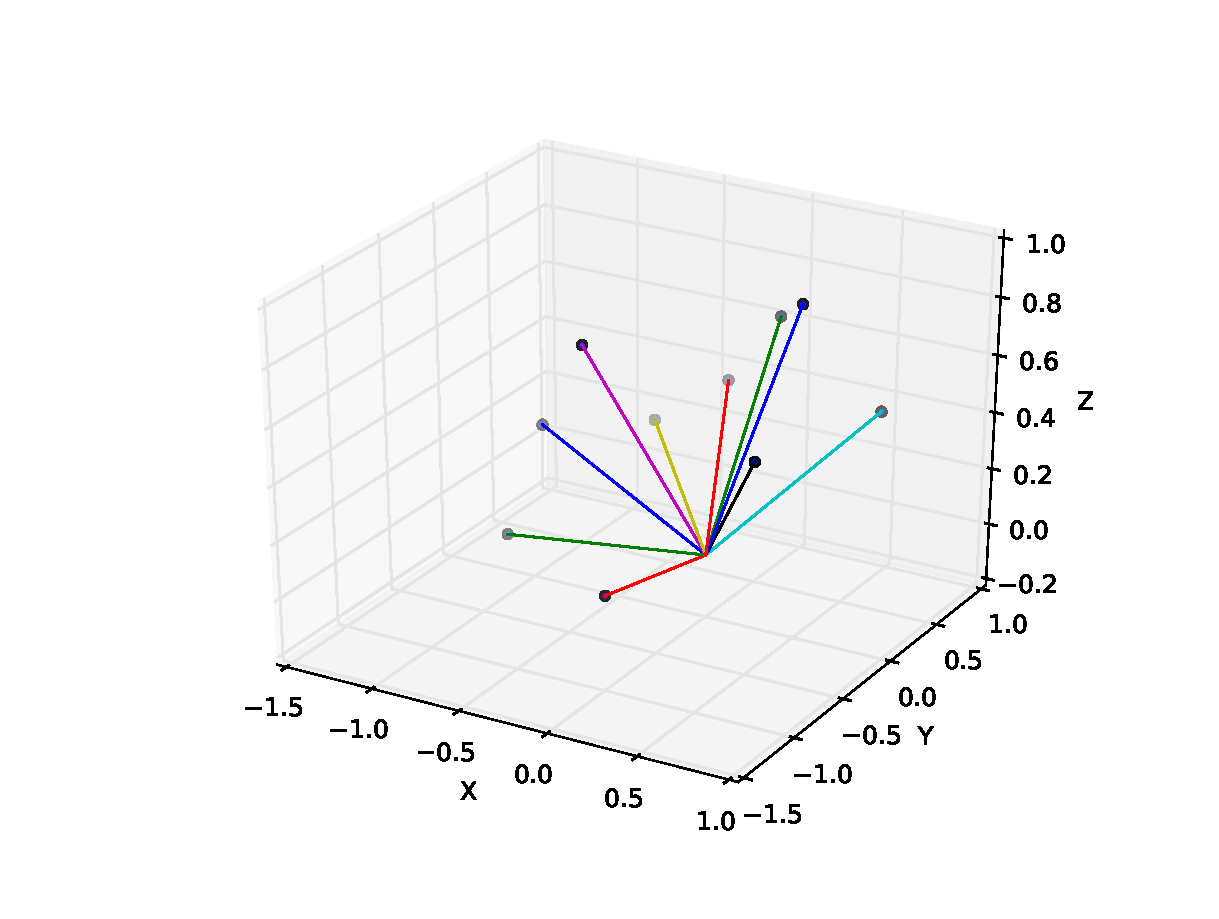
\includegraphics[height=0.7\textheight]{freulon_algo_10_bands.pdf}
\end{center}
\caption{10 bands generated using the Freulon's algorithm}
\label{fig:freulon_algo_10_bands}
\end{figure}
\end{frame}


\begin{frame}
\frametitle{Generating the directions}
\begin{figure}
\begin{center}
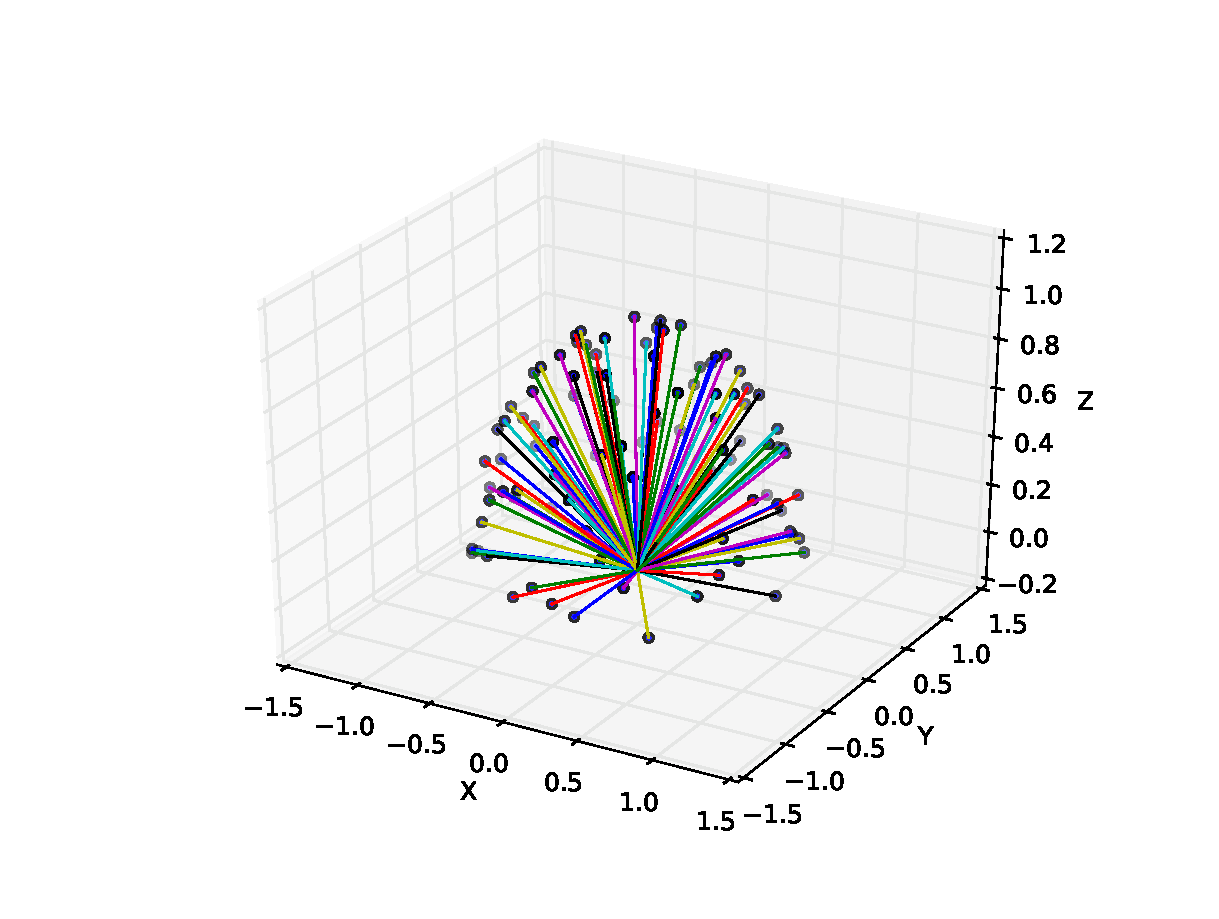
\includegraphics[height=0.7\textheight]{freulon_algo_100_bands.pdf}
\end{center}
\caption{100 bands generated using the Freulon's algorithm}
\label{fig:freulon_algo_100_bands}
\end{figure}
\end{frame}


\begin{frame}
\frametitle{Generating the directions}
\begin{figure}
\begin{center}
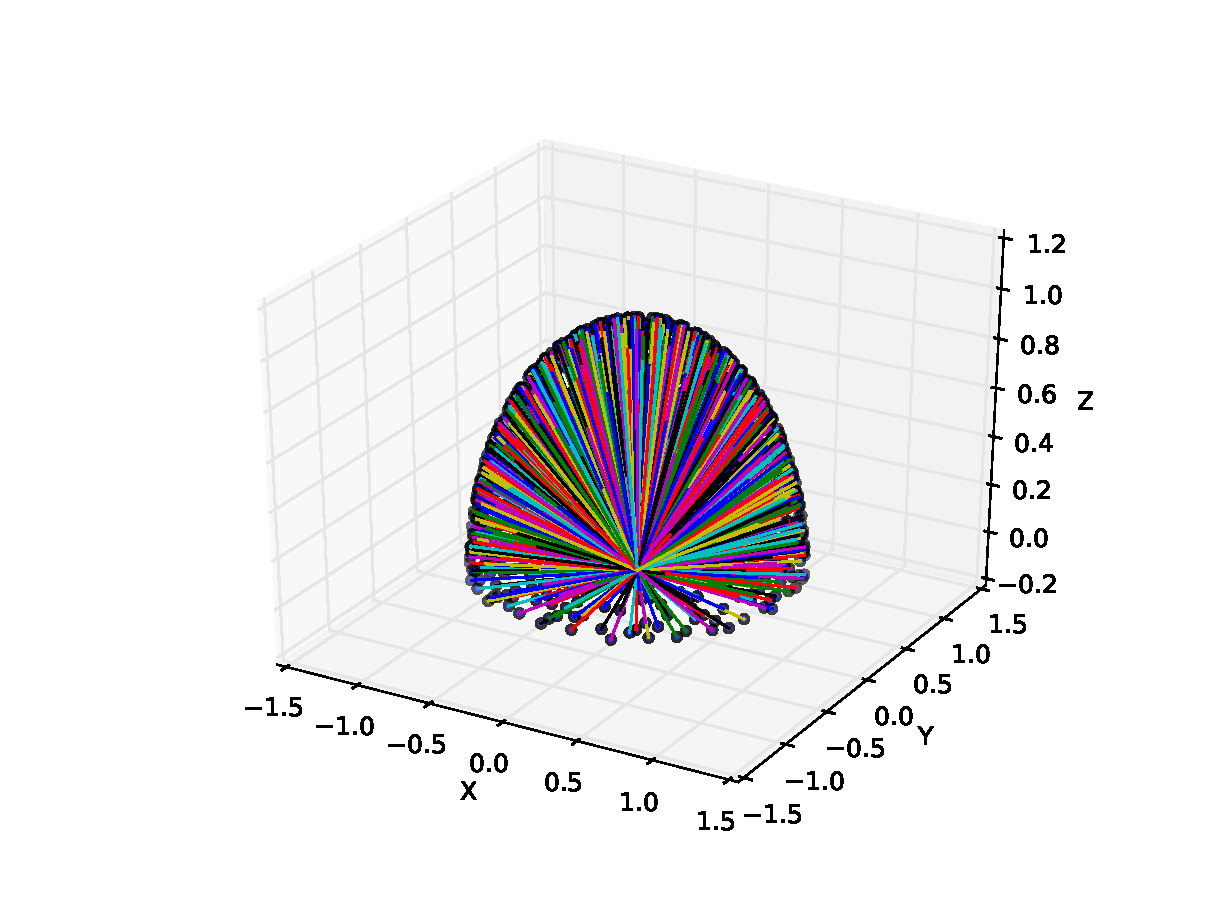
\includegraphics[height=0.7\textheight]{freulon_algo_1000_bands.pdf}
\end{center}
\caption{1000 bands generated using the Freulon's algorithm}
\label{fig:freulon_algo_1000_bands}
\end{figure}
\end{frame}


%%%%%%%%%%%%%%%%%%%%%%%%%%%%%%%%%%%%%%%%%%%%%%%%%%%%%%%%%%%%%%%%%%%%%%%%%%%%%%%%%%%%%%%%%%%%%%%%%%%%%%%%%%%%%%%%
\subsection{Generating the unidimensional simulations}

\begin{frame}
 \frametitle{Generating the unidimensional simulations}
 Now, we have a solution to generate the bands to fill the unit sphere in $\mathbb{R}^3$. But, we have other problem:
 how to generate in each band a stochastic process with covariance function $C_1$?
\end{frame}

\begin{frame}
 \frametitle{Generating the unidimensional simulations}
 
 The Turning Bands algorithm doesn't determine an algorithm to generate the independent stochastic process in each band. 
 Hence, in practice, for each model and band we generate independently the stochastic process using the appropriated 
 algorithm to the specific model. After the execution of all independent simulations in a direction $\theta_n$, 
 the results are linearly combined to generate the final result in this direction. \cite{e2006} presents 15 algorithms
 to generate 15 different types of Covariance models.
 
 In this presentation, we will present just the 3 models: nugget, spherical and the Gaussian.
\end{frame}


\begin{frame}
 \frametitle{Generating the nugget covariance}
 To generate a stochastic process with a covariance that is the spectral representation of the nugget covariance is enough to
 generate a random number with Gaussian distribution $N(0, C)$ with mean 0 and variance C.
\end{frame}


\begin{frame}
 \frametitle{Generating the spherical covariance}
   The algorithm to generate the stochastic process associated to the \textit{Spherical covariance} 
   \begin{equation}
    C_y(r) = C(1-\frac{3r}{2a} + \frac{r^3}{2a^3})1_{0\leq r \leq a}
   \end{equation}
   
   with sill $C$ and range (scale factor) $a$ is
   
   \begin{block}{Algorithm to generate a stochastic process with spherical covariance}
    \begin{enumerate}
     \item choose an offset on the real axis at random
(uniformly in $[0,a[$) and divide this axis in
intervals with length $a$.
      \item within each interval, draw a linear function with
an equal probability of being increasing or
decreasing; the slope sign is independent from
one interval to another one.
       \item the slope value is $2 \sqrt{\frac{3 C}{n}} $, where $n$ is the number of bands.
    \end{enumerate}

   \end{block}


\end{frame}


\begin{frame}
 \frametitle{Generating the spherical covariance}

 \begin{figure}
\begin{center}
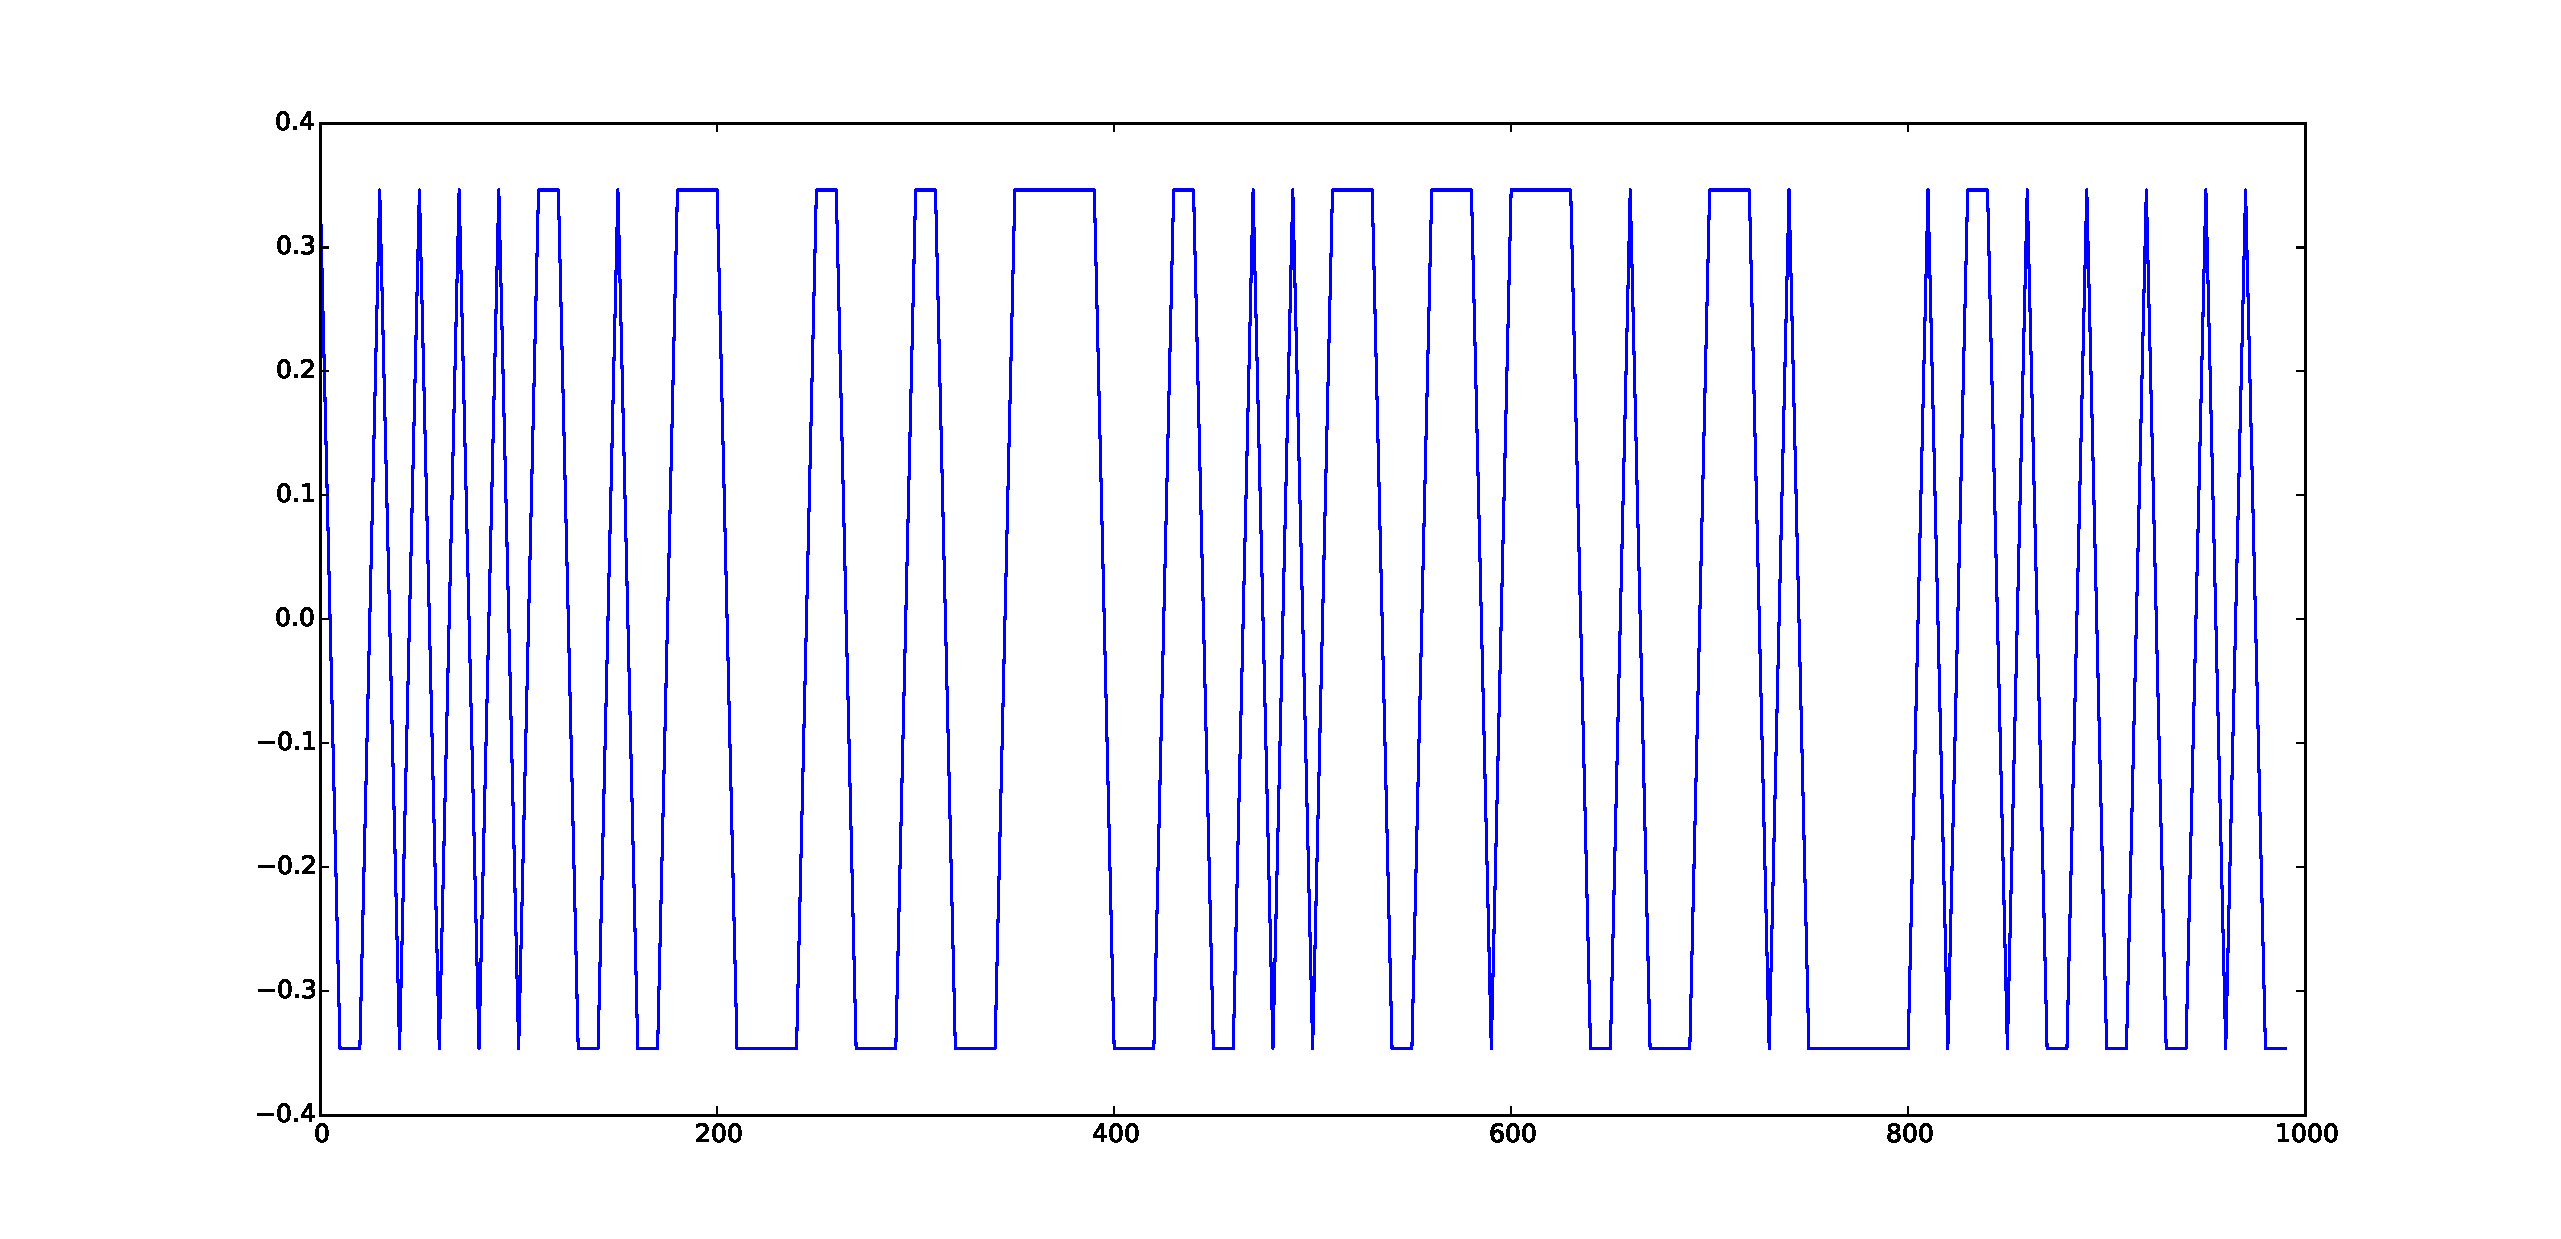
\includegraphics[width=0.8\textwidth]{sthocastic_simulation_spherical.pdf}
\end{center}
\caption{Simulation of the stochastic process associated to the \textit{Spherical covariance} with $C = 10$, $a = 10$}
\label{fig:sthoc_spherical_simulation}
\end{figure}

 
\end{frame}


\begin{frame}
 \frametitle{Generating the spherical covariance}
 
\begin{figure}
\begin{center}
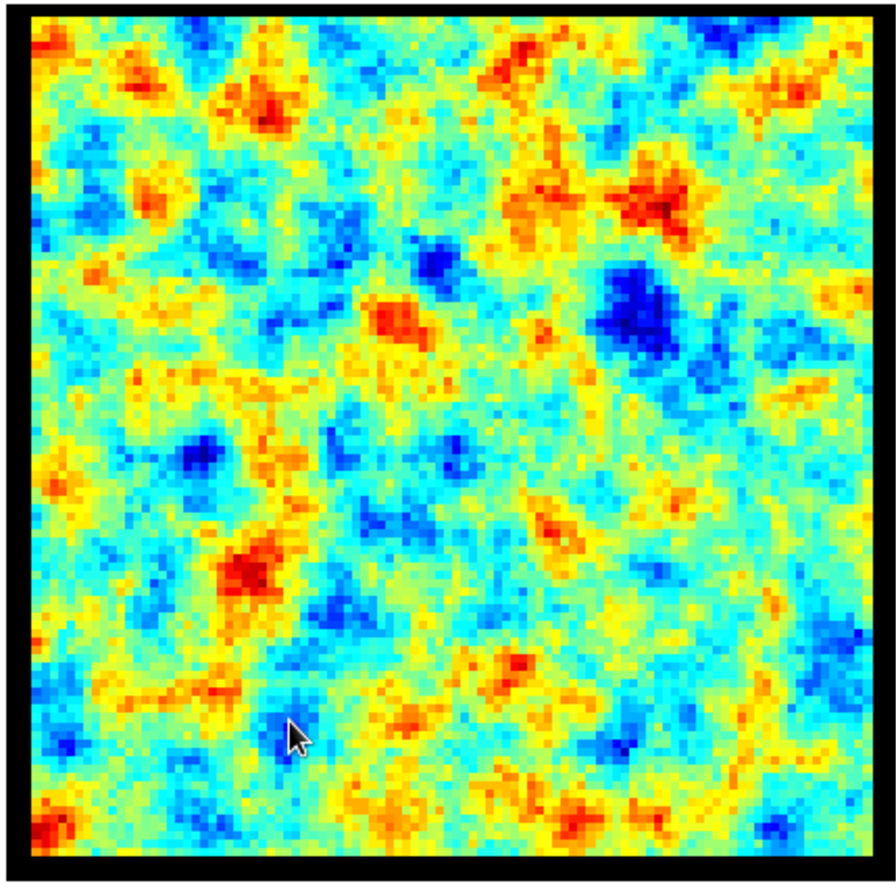
\includegraphics[width=0.5\textwidth]{spherical_simulation_a=10_C=10.pdf}
\end{center}
\caption{Unconditional simulation using a \textit{Spherical covariance} with $C = 10$, $a = 10$ and 1000 lines.}
\label{fig:spherical_unc_simulation}
\end{figure}
\end{frame}

\begin{frame}
 \frametitle{Generating the Gaussian covariance}
 
 We can use the continuous spectral method \cite{e2006} to generate the associated stochastic process to the \text{Gaussian covariance}
 \begin{equation}
  C_Y(r) = C \exp\left\{-\left(\frac{r}{a}\right)^2\right\}
 \end{equation}

 with sill $C$ and scale factor $a$ (practical range $a\sqrt 3$). The algorithm is the following:
 
 \begin{enumerate}
  \item Generate a Gaussian vector $T$ and an uniform random phase $\phi$ defined in $[0,2\pi[$. In $\mathbb{R}^3$, the Gaussian vector can be computed
  as $T=(t_1, t_2, t_3)$, where $t_i, i = 1, 2, 3$ is a Gaussian random number with distribution $N(0,1)$.
  \item The stochastic process is simulated using the equation 
  $Y_\theta(X) = \sqrt{2C} \cos(2\pi(<x, T> + \phi))$, 
  where $X \in \mathbb{R}^3$.
 \end{enumerate}

 
\end{frame}


\begin{frame}
 \frametitle{Generating the Gaussian covariance}
 
\begin{figure}
\begin{center}
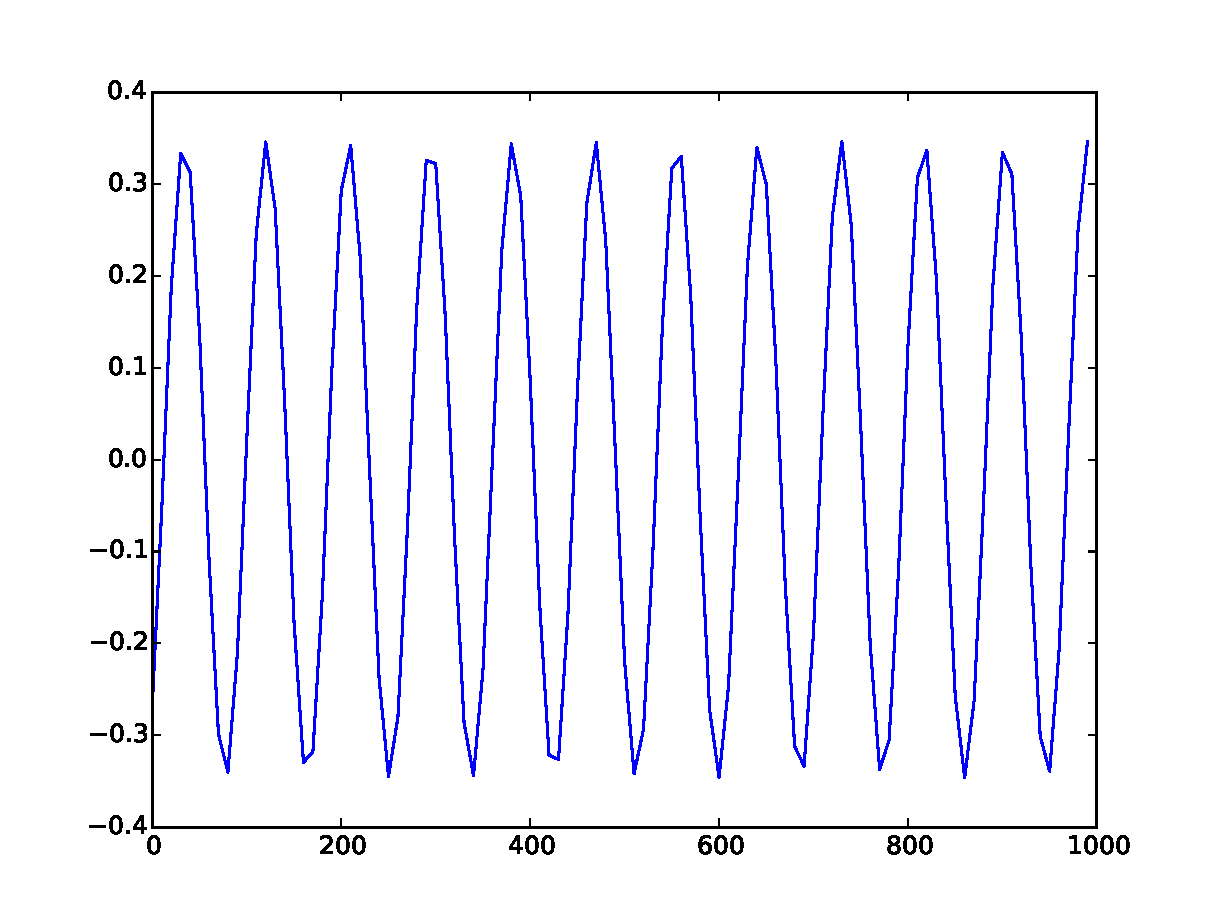
\includegraphics[width=0.5\textwidth]{sthocastic_simulation_gaussian.pdf}
\end{center}
\caption{Simulation of the stochastic process associated to the \textit{Gaussian covariance} with $C = 10$, $a = 10$}
\label{fig:sthoc_gauss_simulation}
\end{figure}
\end{frame}

\begin{frame}
 \frametitle{Generating the Gaussian covariance}
 
\begin{figure}
\begin{center}
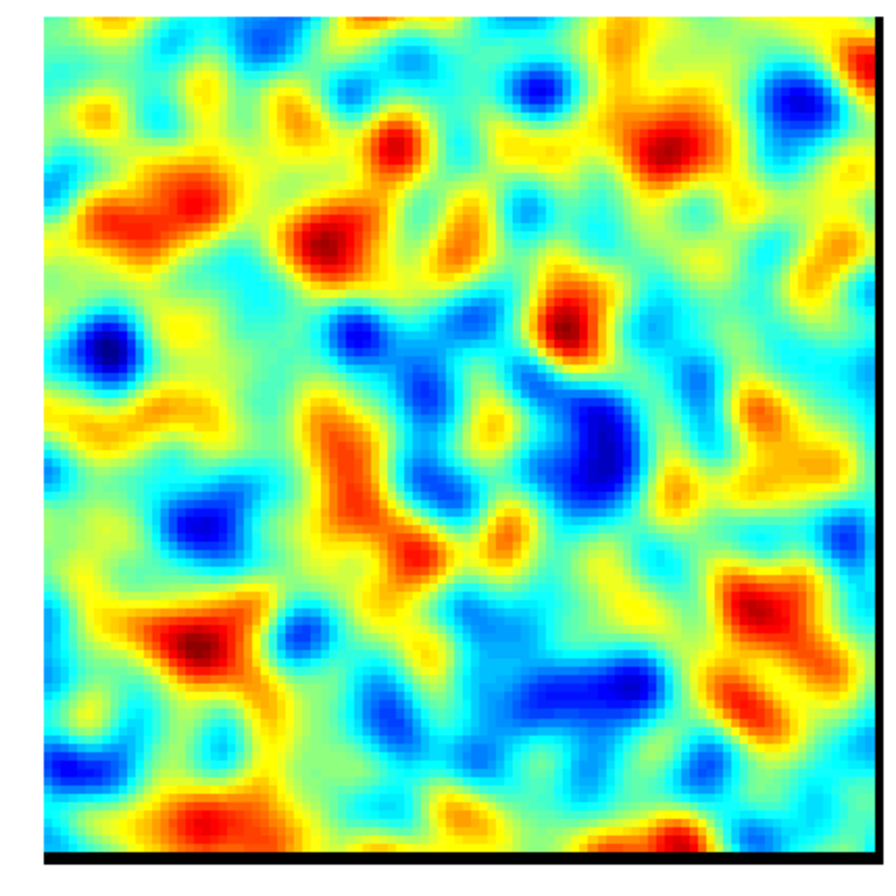
\includegraphics[width=0.5\textwidth]{gaussian_simulation_a=10_C=10.pdf}
\end{center}
\caption{Unconditional simulation using a \textit{Gaussian covariance} with $C = 10$, $a = 10$ and 1000 lines.}
\label{fig:gaussian_unc_simulation}
\end{figure}
\end{frame}


\subsection{Conditioning the simulations}

\begin{frame}
\frametitle{Conditioning the simulations}
 In the previous slides, we presented some techniques to simulated the stochastic process associated with some types of covariances. Now,
 we will present the algorithm to generate the conditional simulations using Turning Bands (or other type of algorithm)
 in the simulation domain $D$ \cite{l2002}. 
 In this algorithm, $CD$ stands the conditioning data-set.
 
\begin{block}{Conditional simulation of a Gaussian Random Function}
 \begin{enumerate}
  \item Calculate the kriged estimates $y^{*}(x)=\sum_c\lambda_c(x)y(c)$ for each $x \in D$.
  \item Simulate a gaussian random function (using Turning Bands or other type of simulation algorithm) with mean $0$ and covariance $C$
  in the domain $D$ and at the conditioning points. Let ($z(x), x \in D$) and ($z(c), c \in CD$) be the generated values.
  \item Calculate the kriged estimates $z^{*}(x) = \sum_c\lambda_c(x)z(c)$ for each $x \in D$.
  \item Return ($y^{*}(x) + z(x) - z^{*}(x), x \in D$).
 \end{enumerate}

\end{block}

\end{frame}


\section{Final Remarks}
\begin{frame}
 \frametitle{Final Remarks}
 \begin{itemize}
  \item From the operational point of view, the Turning Bands is very similar to other Gaussian simulation algorithms like the
  \textit{Sequential Gaussian Simulation}. The only difference is the parameter \textit{number of lines (bands)}.
  \item The quality (convergence velocity) of the Turning Bands is directly related to the number of lines and to the algorithm
  used to generated the band directions.
  \item In the practice, using the Freulon's algorithm, a number of lines greater than 1000 is enough to generate good results \cite{e2006}.
  \item When the number of lines is not appropriated, artifacts are generated.
  \item The Turning Bands is a \textit{share nothing} algorithm, so it's very easy to implement a highly efficient distributed version
  of this algorithm. The SGeMS has a very good implementation using openMP.
 \end{itemize}
\end{frame}

\begin{frame}
 \frametitle{Final Remarks}
 
\begin{figure}
\begin{center}
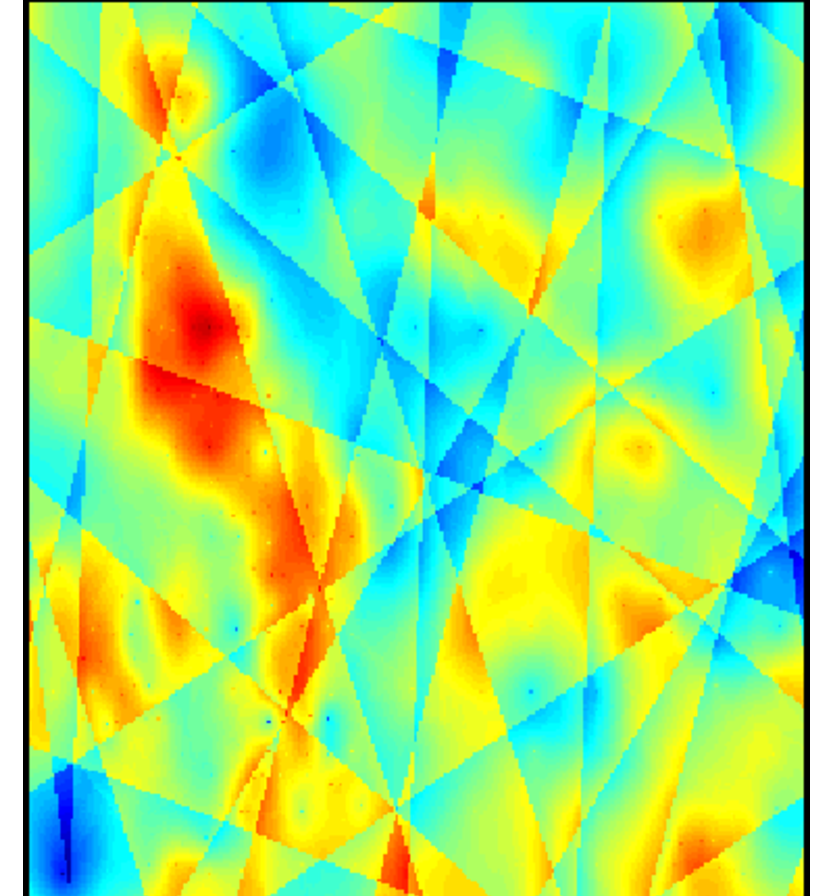
\includegraphics[width=0.5\textwidth]{walker_lake_tb_n=10.pdf}
\end{center}
\caption{Conditional simulation of the Walker lake data-set with number of lines equals to 10.}
\label{fig:gaussian_unc_simulation}
\end{figure}
\end{frame}

\begin{frame}
 \frametitle{Final Remarks}
\begin{figure}
\begin{center}
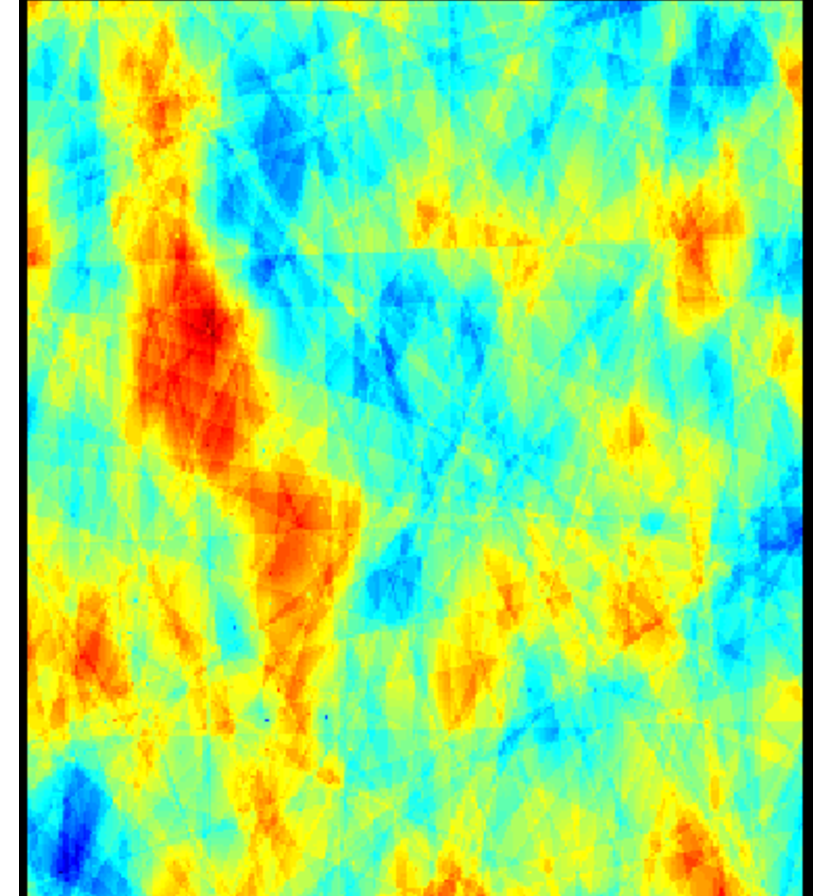
\includegraphics[width=0.5\textwidth]{walker_lake_tb_n=100.pdf}
\end{center}
\caption{Conditional simulation of the Walker lake data-set with number of lines equals to 100.}
\label{fig:gaussian_unc_simulation}
\end{figure}
\end{frame}

\begin{frame}
 \frametitle{Final Remarks}
\begin{figure}
\begin{center}
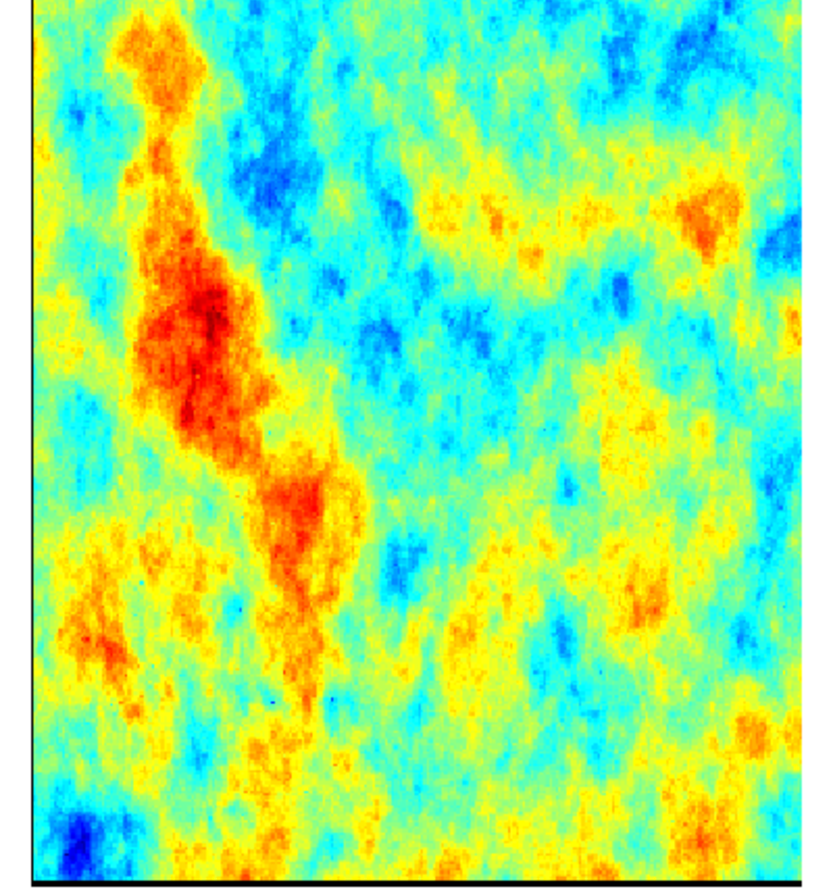
\includegraphics[width=0.5\textwidth]{walker_lake_tb_n=1000.pdf}
\end{center}
\caption{Conditional simulation of the Walker lake data-set with number of lines equals to 1000.}
\label{fig:gaussian_unc_simulation}
\end{figure}
\end{frame}

%%%%%%%%%%%%%%%%%%%%%%%%%%%%%%%%%%%%%%%%%%%%%%%%%%%%%%%%%%%%%%%%%%%%%%%%%%%%%%%%%%%%%%%%%%%%%%%%%%%%%%%%%%%%%%%%
\begin{frame}
\frametitle{References}
\footnotesize{
\begin{thebibliography}{99} % Beamer does not support BibTeX so references must be inserted manually as below
\bibitem[Lantuéjoul, 2002]{l2002} Christian Lantuéjoul (2002)
\newblock Geostatistical Simulation  - Models and Algorithms
\newblock \emph{Springer}, ISBN 3-540-42202-1

\bibitem[Emery, 2006]{e2006} Xavier Emery, Christian Lantuéjoul (2006)
\newblock TBSIM: A computer program for conditional simulation of three-dimensional Gaussian random fields via the turning bands method
\newblock \emph{Computer and Geosciences 32}, Elsevier, 2006, 1615-1628pp, 

\bibitem[Matheron, 1973]{m1973} G. Matheron (1973)
\newblock The Intrinsic Random Functions and Their Applications
\newblock Advanced Applications probability

\bibitem[Freulon, 1994]{f1994} Xavier Freulon (1994)
\newblock Conditional simulation of a Gaussian random vector with non linear and/or noisy observations
\newblock Geostatistical Simulations, Kluwer, Dordrecht, 57-71.
\end{thebibliography}
}
\end{frame}

%------------------------------------------------

\begin{frame}
\Huge{\centerline{The End}}
\end{frame}

%----------------------------------------------------------------------------------------

\end{document} 


